\documentclass{article}
% if you need to pass options to natbib, use, e.g.:
%     \PassOptionsToPackage{numbers, compress}{natbib}
% before loading neurips_2020

% ready for submission
% \usepackage{neurips_2020}

% to compile a preprint version, e.g., for submission to arXiv, add add the
% [preprint] option:
%     \usepackage[preprint]{neurips_2020}

% to compile a camera-ready version, add the [final] option, e.g.:
    \usepackage[final]{neurips_2020}

% to avoid loading the natbib package, add option nonatbib:
    %  \usepackage[nonatbib]{neurips_2020}

\usepackage[utf8]{inputenc} % allow utf-8 input
\usepackage[T1]{fontenc}    % use 8-bit T1 fonts
\usepackage{hyperref}       % hyperlinks
\usepackage{url}            % simple URL typesetting
\usepackage{booktabs}       % professional-quality tables
\usepackage{amsfonts}       % blackboard math symbols
\usepackage{nicefrac}       % compact symbols for 1/2, etc.
\usepackage{microtype}      % microtypography
\usepackage{enumitem}
\usepackage{graphicx}
\usepackage{float}

\title{Playing Competitive Pokémon with DQNs}

\author{%
  Ozaner Hansha \\
  B.S. Computer Science\\
  Rutgers University\\
  New Bruinswick, NJ 07928 \\
  \texttt{ozaner.hansha@rutgers.edu} \\
}

\begin{document}

\maketitle

\begin{abstract}
  Pokémon is a popular RPG video game franchise with a similarly popular competitive scene. The mechanics of Pokémon present an interesting challenge and testbed for reinforcement learning methods. In this paper, we desmonstrate the viability of using Deep Q Networks, as described by Mnih, Kavukcuoglu, et al. [1], for this problem by training one as a battling agent. The resulting DQN agent was tested against a ubiquitous baseline strategy in Pokémon battling, expected damage maximization, and is capable of performing better than it. This suggests that DQN based Pokemon agents are viable against human opponents.
\end{abstract}

\section{Introduction}
The Pokémon series of video games has two core mechanics, catching Pokémon and battling with those Pokémon against either in game AI or real life players. These `Pokémon' are creatures in the game, each with widely varying attributes and abilities (attack, defense, health points, moves, etc.). These varying characteristics can result in complex strategies, dependent on how they interact. This fact, combined with the huge popularity of Pokémon and its resultingly large player base, makes Pokémon battling an ideal, yet underused, testbed for reinforcement learning methods.

In this paper, we present a Pokémon battling agent based off of a Deep Q Network (DQN) as described in \textit{Human-level control through deep reinforcement learning} [1]. Our network is trained by directly partaking in battles against other agents on Pokémon Showdown [3], a Pokémon battle simulator in which much of the competitive scene takes place.

In particular, our agent will be competing in the \texttt{gen8randombattle} format. As in the name, the Pokémon the AI will have access to are all those available in generation 8 of the Pokémon games (i.e. the most recent as of writing) but crucially, these Pokémon will be chosen at random for both the player and opponent. This serves both as a simplification of the problem and generalization for our agent as it now only has the task of learning how to battle in general and not of battling with a specific team.

We aim to show, via the DQN agent, the viability of using reinforcement learning techniques to tackle to problem of Pokémon battles, as well as provide insight steps forward to improve results on this task.

\section{Related Works}
There have been a few papers on this problem using classical solutions, like the minimax algorithm, as well as reinforcement algorithms, like shallow Q-learning [5] [6]. While most of these papers have agents learn in different formats to the one we are using, and in particular train their agents with specific teams rather than random ones, their results show win rates hovering around 60-65\% against the baseline strategy of picking the highest damaging moves.

It seems the challenge in fitting or training a Pokémon battling agent is giving it a large quantity of relevant battle examples, presumably ones with a high self-information, although we do not formalize this notion for Pokémon battles. The complexity of Pokémon battles, and thus their strategies also plays a large role in building battle agents. It would appear that the agents proposed in previous works were not complex enough to fit or learn these strategies even if given lots of high information samples. 

\section{Main Contribution}
As mentioned in the previous section, the two key challenges that a Pokémon battle agent must address are and increase in its model complexity, as well as an increase in its training data to accompany that higher complexity.

We solve the problem of model complexity compared to past approaches by, quite simply, adding more layers to our Q-learning algorithm, netting us a DQN.

We approach the more difficult problem of obtaining enough training data to fit said model in a two-fold approach:
\begin{enumerate}[label=(\alph*)]
  \item We have our model connect to the official Pokémon Showdown server, allowing it to train and evaluate itself against real players on the ladder.
  \item Instead of having our baseline agent be one that picks the move with the highest base power, regardless of the context, we instead created our own baseline that is more accurate to the strategy of the game. This agent greedily chooses the move that maximizes the expected damage against the current opponent Pokémon. We call this the expected damage maximization (EDM) agent.
  \item Rather than train our model solely against human players or a baseline agent, we bootstrap it's training by having it train on both. First we have it train on the baseline agent until it converges in performance, then we have it train against human players until it converges, or as long as we have time for.
\end{enumerate}

Point (a) gives us more interesting and indeed relevant training data as, in a sense, battles against real people are sampled from the true probability distribution we are seeking to fit, rather than the surrogate one of battles against the baseline agent.

Despite still being a surrogate, point (b) gives us a much better baseline agent to train against. Achieving good performance on the EDM necessitates the DQN to learn the type matchups between the opponent Pokémon and their own. This forces the network to learn more about the mechanics of the game if it is to converge towards a policy against this agent. 

Point (c) allows us to make use of the data from point (a) more effectively. Collecting samples from real battles is much more time consuming than on battles with agents. On top of this, if those battles are against a newly initialized DQN, they are very uniformative as the DQN agent would play just as well as a random agent. By first training our DQN on the baseline, something that is comparatively much less expense, it can stand a fighting chance against real players. This both prevents us wasting time on training with uninformative battles as well as allows the DQN to probe the opponent as it is not hopelessly outclassed.

Connecting to showdown was possible via an open source library for creating Pokémon RL agents called Poke-env [2]. It serves as a wrapper for Showdown as well as comes with an implementation of an environment from open-ai's gym package for RL [8].

\section{Experiment}
\subsection{DQN Model \& Training Algorithm}
We set up our DQN to take in 10 features, elaborated on below, and put them through 2 fully connected layers with ReLu activation and a final output layer with a linear activation function. The output of this network is 22 dimensional, representing the 22 different options available to a player. The model is given graphically below:

\begin{figure}[H]
  \centering
  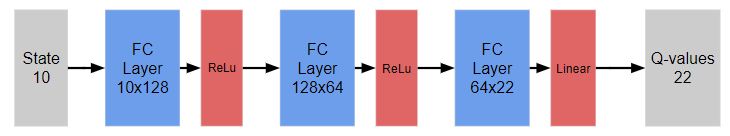
\includegraphics[scale=.7]{dqn.png}
  \caption{The DQN model used in the experiment.}
\end{figure}

We train our DQN with the standard approach of sampling random batches from replay memory as well as having both a policy and target net:

\begin{figure}[H]
  \centering
  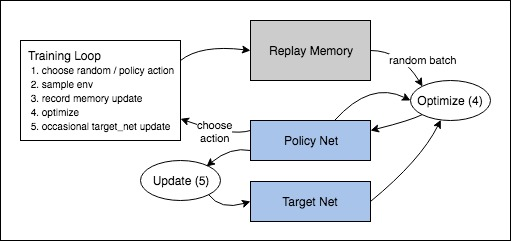
\includegraphics[scale=.7]{dqn-train.jpg}
  \caption{The DQN training loop.}
\end{figure}

\subsection{Features \& Rewards}
At each observation phase, we give our DQN the following 10 features:
\begin{enumerate}
  \item \# of remaining Pokémon on team
  \item \# of remaining Pokémon on opponent's team
  \item Base power of current Pokémon's move 1\\\setcounter{enumi}{5}
  $\vdots$
  \item Base power of current Pokémon's move 4
  \item Damage multiplier of current Pokémon's move 1\\\setcounter{enumi}{9}
  $\vdots$
  \item Damage multiplier of current Pokémon's move 4
\end{enumerate}

This is a very simple feature set, but its simplicity facilitates faster learning. The rewards we give to the agent are as follows:
\begin{itemize}
  \item 30 reward for winning.
  \item $.01x$ for removing $x$\% of an opponent Pokémon's health.
  \item 1 reward for knocking out an opponent Pokémon.
\end{itemize}

Note that for the second bullet point, the reward is scaled with respect to the opponent Pokémon's total health. 

\subsection{Training}
We first trained the DQN agent against the EDM agent, until the loss appeared to converge. We then performed early stopping and reverted the network to when convergence first started, this was at about 12000 iterations:

\begin{figure}[H]
  \centering
  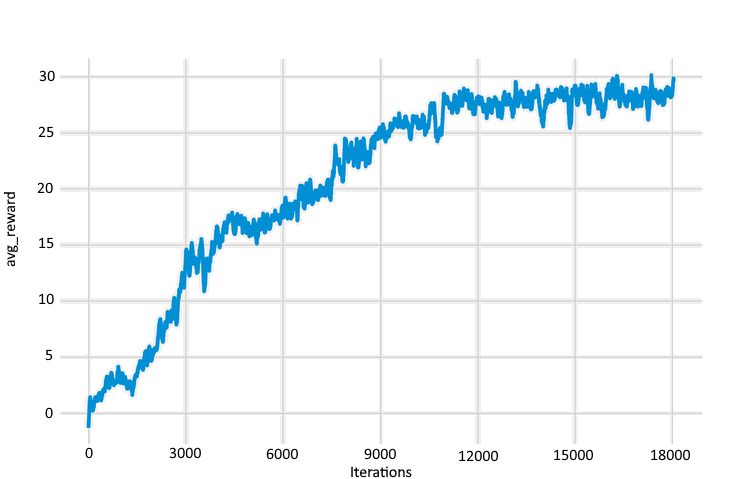
\includegraphics[scale=.7]{training.png}
  \caption{Reward over time while training against EDM.}
\end{figure}

After this, we connected the to showdown via \texttt{poke-env} to train against real human players. The DQN agent played 712 matches online, although we would ideally have it done more.

\subsection{Results}
To evaluate the agent after training on both EDM and human agents, as well as have some comparison we had three agents play 500 matches against each other. These bots are:
\begin{itemize}
  \item Random Agent: picks one of the available 22 actions with uniform probability.
  \item EDM Agent: picks the action that greedily maximizes the expected damage.
  \item DQN Agent: the agent in question based off of a Deep Q network.
\end{itemize}

Here are the results, note that we did evaluate test the bots on themselves hence the empty diagonals:
\begin{center}
  \begin{tabular}{||c c c c||} 
  \hline
  Agent & Random & EDM & DQN \\ [0.5ex] 
  \hline\hline
  Random & - & 0.6\% & 1.7\% \\ 
  \hline
  EDM & 99.4\% & - & 27.4\% \\
  \hline
  DQN & 98.3\% & 72.6\% & - \\
  \hline
 \end{tabular}
\end{center}

The table above shows the win-rate of the 500 matches of the row against the column. As we can see, both the EDM and DQn agents trounced the random agent, which is to be expected. Indeed if they couldn't do this then it would be clear they don't represent meaningful strategies at all.

More interestingly is that the DQN defeated the EDM with a 72.6\% win-rate. This beats other papers [5] [6] results against the baseline and points to even greater potential performance of the DQN given more resources and data.

We also tested how the DQN fares against human palyers. After testing on 324 different human matches with random players over the course of two days we have that the DQN beat the humans 68.3\% of the time. Note however that Showdown matches players up based on their ELO rating. A more accurate measure of the bot's performance may be the ELO rating itself which reached a 1353 ELO. Showdown's ELO rating is modified however [8], as it includes a decay factor and other factors to discourage players from not playing to maintain their rating. This is all to say that more evaluation has to be done to gauge accurate results about the agent against humans in general.

\section{Conclusion}
Our DQN agent shows promoising results considering its feature vector was filled with only basic information about the state of the battle. More nuanced feature observations (e.g. Pokémon usage, auxillary effects of moves, and even typings of opponent Pokémon as they become available) about the environment may lead to more nuanced strategies which can make a huge difference in win-rate with such an adversarial game.

That said, there are other models that could serve as viable alternatives to DQNs. Policy gradient (PG) methods are one such model. On policy learning is known to better avoid local minimums compared to the off policy learning of DQNs. PGs, however, still must deal with the problem of obtaining training data and this problem is compounded by the fact that they often need more data to converge upon a good solution. [7] Actor-critic models may serve to be the best of both worlds in that respect, by both being on-policy and requiring less data to converge. However this is a claim to be verified by experiment.

What has also become clear is that, while the EDM baseline is not perfect and cannot make use of complex strategies like poisining the opponents team, it still serves as a very good objective in training as well as general benchmark for any Pokémon battle agent. Heuristically speaking, being able to beat such an agent with a high win-rate, say around 85-90\%, seems to be a prerequisite for agents to be able to take on (and make use of) training data gathered from real battles.

\section*{References}
\small
[1] Mnih, Kavukcuoglu, et al. Human-level control through deep reinforcement learning\\
\texttt{https://web.stanford.edu/class/psych209/Readings/MnihEtAlHassibis15NatureControlDeepRL.pdf}

[2] Haris Sahovic, et al. \texttt{poke-env}. \\
\texttt{https://github.com/hsahovic/poke-env}

[3] Smogon. \texttt{pokemon-showdown}. \\
\texttt{https://github.com/smogon/pokemon-showdown}

[4] Bulbapedia. \texttt{https://bulbapedia.bulbagarden.net/wiki/Pokémon\_battle}

[5] Rill-García. Reinforcement Learning for a Turn-Based Small Scale Attrition Game\\
\texttt{https://ccc.inaoep.mx/~esucar/Clases-mgp/Proyectos/2018/reinforcement-learning-turn\%20\%281\%29.pdf}

[6] Kalose, Kaya, Kim. Optimal Battle Strategy in Pokémon using Reinforcement Learning\\
\texttt{https://web.stanford.edu/class/aa228/reports/2018/final151.pdf}

[7] Yu. Deep Q Network vs Policy Gradients - An Experiment on VizDoom with Keras\\
\texttt{https://flyyufelix.github.io/2017/10/12/dqn-vs-pg.html}

[8] Brockman, et al. \texttt{OpenAI Gym}\\
\texttt{https://github.com/openai/gym}

[9] Antar. \texttt{Everything You Ever Wanted to Know About Ratings}\\
\texttt{https://www.smogon.com/forums/threads/everything-you-ever-wanted-to-know-about-ratings.3487422/}

\end{document}